\chapter{\label{method}Improving the Bucket with Global Query-algorithm}

\iffalse

\textbf{The Company}  Something about a a very common business model (small startup, free-to-play) limited budget and business not large enough to run server park on its own.

\textbf{The Application} Game, number of users

\textbf{Infrastructure} The backend handling the highscores and rankings runs on Google App Engine (GAE) which is a Platform-as-a-Service-cloud service (PaaS). The current system is implemented in Java.

Since applications running on GAE do not have access to a file system, data is stored in the App Engine Datastore which is NoSQL key-value-store. While the application part of the GAE scales automatically as far as the configuration allows, the throughput when writing to the same object in the Datastore is very limited and measures need to be taken to avoid cogestion. 

Finally a service provided by the GAE worth mentioning is the memory cache. The Memory cache or memcahce is provided at different service levels, paid and free, the later without any guarantees at all. The memcache may be used for keeping the number of reads from the datastore at a minimum. It is however not durable and cache-misses needs to be handled gracefully.

\fi

\todo{Background}

The Companys current ranking algorithm is an implementation of the algorithm \emph{Bucket with Global Query} (See \labelcref{bucket}). The highscores are stored in Google App Engines Datastore as entities with properties \emph{username} and a \emph{highscore}. When a player gets a new highscore it replaces the old highscore. Note that this implies that highscore entries never will get updated with a lower score than previously recorded for that user.

Since score in this case is measured in milliseconds and lower timings are better a better score is a lower number.

\section{Hypothesis} 

The current implementation starts a background job that builds the bucket-table every ten minutes. When the scan is complete a reference is set to the new table and the old one is discarded. The error is a priori assumed to be at its maximum level right before the switch (See figure \ref{fig:errortime}) and will in the forthcoming reasonings serve as an upper limit for what would be an acceptable performance.

The total cost for providing the ranking service with the current implementation and the implementation to be assessed is

\begin{equation}
  n \times C_{estimate} + \frac{ C_{table}}{n}
\end{equation}
\todo{Create better formula. Maybe total cost = function(num-estimates, table-recreation-frequency, cost-estimate, cost-table-recreation)}

where $n$ is the number of approximations made, $C_{estimate}$ is the execution time for making one estimate and $C_{table}$ is the cost for recreating the bucket-table.

In the original Bucket with Global Query-algorithm, getting an approximate rank is a lookup-operation in a table (or similar operation on another data structure) and some simple arithmetics, hence the execution time cannot really be improved for that part. The cost for creating a bucket-table can not be radically improved either because it has to iterate over the set of highscores. But if the lifetime of the bucket-table could be extended, its addition to the cost per rank estimate would get lower. As shown in section \ref{bucket}, the bucket-table in use starts to deviate from a true bucket-table when new highscores comes in. The tables score ranges, start ranks and bucket sizes simply don not correspond to the actual set of highscores.

So what if the table's buckets were adjusted when a new highscore gets registered? The overhead caused by aadjusting start ranks and bucket sizes will be small because it can be accomplished in a few lines of code, mostly concerned with increasing and decreasing integer primitive values. But there is also an overhead coming from storing the adjusted table which would apply to every single estimate.

To sum up, the cost for approximating the rank for a highscore will be more expensive when also updating the bucket-table, but will the increased cost it be compensated for by the expected increase in lifetime of the bucket-table? The cost for recreating the bucket table will remain the same. Two possible scenarios are sketched in figure \ref{fig:cost}.

\begin{figure}[h]
  \centering
  \caption{Possible scenarios for cost growth.}
  \label{fig:cost}
  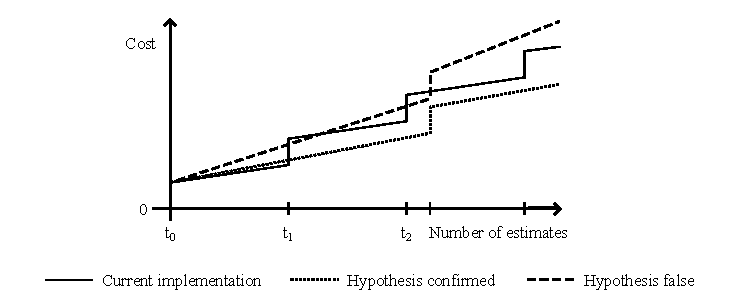
\includegraphics[width=13cm]{img/hypothesis-cost1.eps}
\end{figure} 

The hypothesis reads as follows: \emph{\textbf{Running the ranking service with the new implementation will be more efficient than the current implementation at the same level of error.}}

\section{Data}

In this experiment only synthetic data will be used. The choice is both practical and a methodologically motivated. First, the production system as cannot be altered in such a way that real world data could be tapped within this experiments timeframe. Also, real world data in this system differs from one time period to another both in terms of the highscore distribution and throughput. And of course, data from one application differs from data from other applications. Using synthetic data make the results more general.

Random data is used in two ways. First, the experiment is started with a set of 100 000 highscores having a Gaussian distribution with mean 1 000 000 and variance 1 000 000, also scores below 1000 are not included\footnote{The real world highscores are similarly distributed to each other and somewhat similar to a Gaussian distribution. However, no effort has ben made to do a statistical analysis of them.} (Figure \ref{fig:highscore-distribution}). Second, the improvement for the new highscores used in the experiment are picked from a uniform distribution $\mathcal{U}\{1, 1000\}$.
 
\begin{figure}[h]
  \centering
  \caption{Initial highscore distribution.}
  \label{fig:highscore-distribution}
  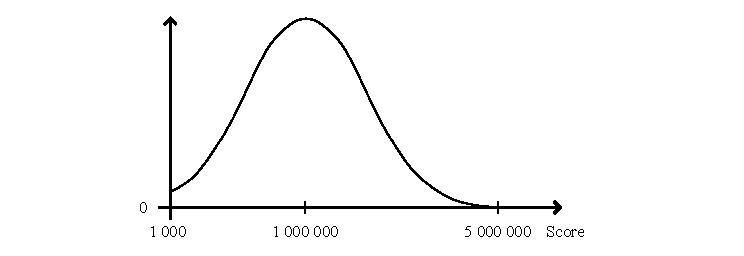
\includegraphics[width=13cm]{img/highscore-distribution.eps}
\end{figure} 

The random number generator in Java is used and is always initialized with the same random seed to achieve repeatability.  

\section{The experiment}

The experiment is implemented in a client-server-model where the client simulate playing a game and sends highscores to the server. The server responds with an approximated rank and the execution time for processing the request. The client is a regular Java program without bells and whistles and the server consists of a number of servlets designed to run on Google App Engine.

The client plays 100 000 rounds for different users, picked at random. They will always get a new highscore, ie they always win. The new highscore is better than the old one by a number drawn from a uniform pseudorandom distribution $1-1000$.

To be able to measure the relative error of the estimates the client starts by asking for a list of all highscores. When the client sends a new highscore to the server, it also updates its local highscore list. When the server responds with the rank estimate for the new score, that estimate is compared with the real rank and ultimately used for calculating the relative error.

\subsection*{Technical details}

Both client and server parts are run on the same physical computer.

Two libraries are used in the project. \textbf{Objectify} provides means for persisting Java objects to the App Engines Datastore. By a few annotations
\footnote{
  \href
      {https://docs.oracle.com/javase/tutorial/java/annotations/index.html}
      {https://docs.oracle.com/javase/tutorial/java/annotations/index.html}
}
to the Java-class (\texttt{@Entity} on the class and \texttt{@Id} on the String or Long field that will be used for creating the key) objects can be saved with a statement like \texttt{ofy().save().entity(theObject)}. On top of providing an easy way for persisting objects, Objectify also handles caching data in the memory cache.
\textbf{Jackson} is a library for parsing JSON-data as well as mapping JSON to Java objects.

\section{What and how to measure}

To be able to test the hypothesis relative error and execution time will be logged per ranking request. As the true value for calculating the relative error, an exact rank is calculated for every approximation.

The execution time is measured by calls to \texttt{System.currentTimeInMillis()} in the servlet receiving the ranking request.


\section{Limitations}

The experiment is only run using a local development server. While there is no obvious reason to believe that the conclusions could be applied to a production environment in the cloud in principle, there may be factors that need to be considered. 
